% Problem 1 - Capacitor Current, Voltage, Power, and Energy (15 points)
\Point{capacitorcurrent}{voltagepower}{9}
\Point{capacitorcurrent}{waveformplots}{6}
\Point{capacitorcurrent}{peakpower}{2}
\Point{capacitorcurrent}{zero}{3}
\begin{mainquestion}{capacitorcurrent}{Capacitor Analysis}

The current $i_C(t)$ through a \qty{200}{\nano\farad} capacitor is shown in the figure below. At $t = 0$, the voltage $v(t)$ is -16 V.

\begin{center}
\includegraphics[width=1.0\textwidth]{current_circuit.png}
\end{center}

% =========================================================
\begin{partquestion}{voltagepower}
{Calculate the voltage, power, and stored energy of the capacitor as a function of time.}

\begin{answer}
The equation that relates the current and the voltage in a capacitor is given by:

\[
i_C(t) = C \frac{dv_C(t)}{dt} \quad \Rightarrow \quad v_C(t) = \frac{1}{C}\int i_C(t)\,dt + v_C(0)
\]

Nothing happens until 1~ms when the current source begins to output 5~mA.
From 1~ms to 3~ms:

\begin{align*}
v_C(t) &= \frac{1}{\num{200e-9}} \int_{0.001}^t \num{5e-3} \,dt' - 16\\
&= \frac{1}{\num{200e-9}} \int_{0}^{t-0.001} \num{5e-3} \,dt' - 16\\
&= (\num{25e3})(t-0.001) - 16 \quad (0.001 \leq t \leq 0.003\text{ s}) \\
v_C(0.003) &= 50 - 16 = \qty{34}{\volt}
\end{align*}

From 3 ms to 5 ms the current is reversed, which should cause the voltage to fall back down to where it started.
\begin{align*}
v_C(t) &= \frac{1}{\num{200e-9}} \int_{0.003}^t \num{-5e-3} \,dt' +34\\
&= \frac{1}{\num{200e-9}} \int_{0}^{t-0.003} \num{-5e-3} \,dt' +34\\
&= (\num{-25e3})(t-0.003) +34 \quad (0.003 \leq t \leq 0.005\text{ s}) \\
v_C(0.005) &= -50 + 34 = \qty{-16}{\volt}
\end{align*}

Consolidating these results gives:

\[
v_C(t) = \begin{cases}
- 16 & t \leq 0.001 \\
\num{25e3} (t - 0.001) - 16 & 0.001 \leq t \leq 0.003 \\
\num{-25e3} (t - 0.003) + 34 & 0.003 \leq t \leq 0.005 \\
- 16 & t \geq 0.005
\end{cases}
\]

The power stored is given by the product of the current and the voltage in the capacitor, that is, $p_C(t) = v_C(t) \cdot i_C(t)$. Therefore, (measuring power in watts):

\begin{align*}
p_C(t) &= \begin{cases}
(- 16)(0) & t \leq 0.001 \\
(\num{25e3} (t - 0.001) - 16)(0.005) & 0.001 \leq t \leq 0.003 \\
(\num{-25e3} (t - 0.003) + 34)(-0.005) & 0.003 \leq t \leq 0.005 \\
(- 16)(0) & t \geq 0.005
\end{cases} \\
&= \begin{cases}
0 & t \leq 0.001 \\
125(t - 0.001) -0.08 & 0.001 \leq t \leq 0.003 \\
125(t - 0.003) -0.17 & 0.003 \leq t \leq 0.005 \\
0 & t \geq 0.005
\end{cases}
\end{align*}

The energy (measured in joules) stored in the capacitor is given by:

\[
E_C = \frac{1}{2} C V^2 = \frac{1}{2}(\num{200e-9}) v_C(t)^2 = (\num{1e-7}) v_C(t)^2
\]

Using the result for the capacitor voltage from before we can determine:

\begin{align*}
E_C(t) &= \begin{cases}
(\num{1e-7})(-16)^2 & t \leq 0.001 \\
(\num{1e-7})(\num{25e3} (t - 0.001) - 16)^2 & 0.001 \leq t \leq 0.003 \\
(\num{1e-7})(\num{-25e3} (t - 0.003) + 34)^2 & 0.003 \leq t \leq 0.005 \\
(\num{1e-7})(-16)^2 & t \geq 0.005
\end{cases} \\
&= \begin{cases}
\num{25.6e-6} & t \leq 0.001 \\
\num{625e6}t - \num{2.05e6}t + 1681 & 0.001 \leq t \leq 0.003 \\
\num{625e6}t - \num{5.45e6}t + 11881 & 0.003 \leq t \leq 0.005 \\
\num{25.6e-6} & t \geq 0.005
\end{cases}
\end{align*}

\end{answer}
\end{partquestion}

% =========================================================
\begin{partquestion}{waveformplots}
{Plot the current, voltage, power, and stored energy to scale versus time so that the relation between each is clear.}

\begin{answer}
Plotting these graphs gives the results below:

\begin{center}
\includegraphics[width=5in]{waveforms.png}
\end{center}

\end{answer}
\end{partquestion}

% =========================================================
\begin{partquestion}{peakpower}
{What is the peak power and at what time $t$ does it occur?}

\begin{answer}
From the graph and our equations it's clear that the peak power (both positive and negative) occurs at \qty{3}{\milli\second} with a value of \qty{170}{\milli\watt}.
\begin{align*}
    p_C(0.003) &= 125(0.003 - 0.001) -0.08 \\
    &= 125(0.002) -0.08 = 0.25 - 0.08\\
    &= \qty{0.170}{\watt}
\end{align*}
\end{answer}
\end{partquestion}

% =========================================================
\begin{partquestion}{zero}
{What is the minimum and maximum energy stored in the capacitor and at which times $t$ do they occur?}

\begin{answer}
The maximum energy will be stored in the capacitor when $|v_C|$ is at its largest, since the energy is computed using the square of voltage. From the graph, it's clear this happens at \qty{3}{\milli\second} when the capacitor has a voltage of \qty{34}{\volt}. We compute the energy as:
\[
E_{C,\text{max}} = \frac{1}{2}CV_C^2 = \frac{1}{2}(\num{2e-7}) (34)^2 = \qty{115.6}{\micro\joule}
\]

The minimum energy is zero! Since the voltage changed from positive to negative during our analysis, sometime in the middle it passed through \qty{0}{\volt}, which would imply $E_C = 0$ at that point. We can solve for that time by either finding the minimum of the energy function, or solving for when the voltage was equal to zero. Here we will solve using the voltage:

\begin{gather*}
\num{25e3} (t_{\text{min,1}} - 0.001) - 16 = 0 \\
t_{\text{min,1}} = \frac{16}{\num{25e3}} + 0.001 \\
t_{\text{min,1}} = 0.00164 = \qty{1.64}{\milli\second}
\end{gather*}

Keep in mind that the energy also drops to zero again when the current reverses from \qty{3}{\milli\second} - \qty{5}{\milli\second}. We can use the other equation to solve for that one:

\begin{gather*}
-\num{25e3} (t_{\text{min,1}} - 0.003) + 34 = 0 \\
t_{\text{min,2}} = \frac{-34}{\num{-25e3}} + 0.003 \\
t_{\text{min,2}} = 0.00436 = \qty{4.36}{\milli\second}
\end{gather*}

\end{answer}
\end{partquestion}


\end{mainquestion}


% Problem 2 - Capacitor Network DC Analysis (24 points)
\clearpage
\Point{capacitornetwork}{networksteadycurrent}{2}
\Point{capacitornetwork}{networksteadyvoltage}{16}
\Point{capacitornetwork}{energy}{6}
\begin{mainquestion}{capacitornetwork}{DC Capacitor Network}

Consider a network of ten capacitors arranged between two nodes A and B as shown below.

\begin{center}
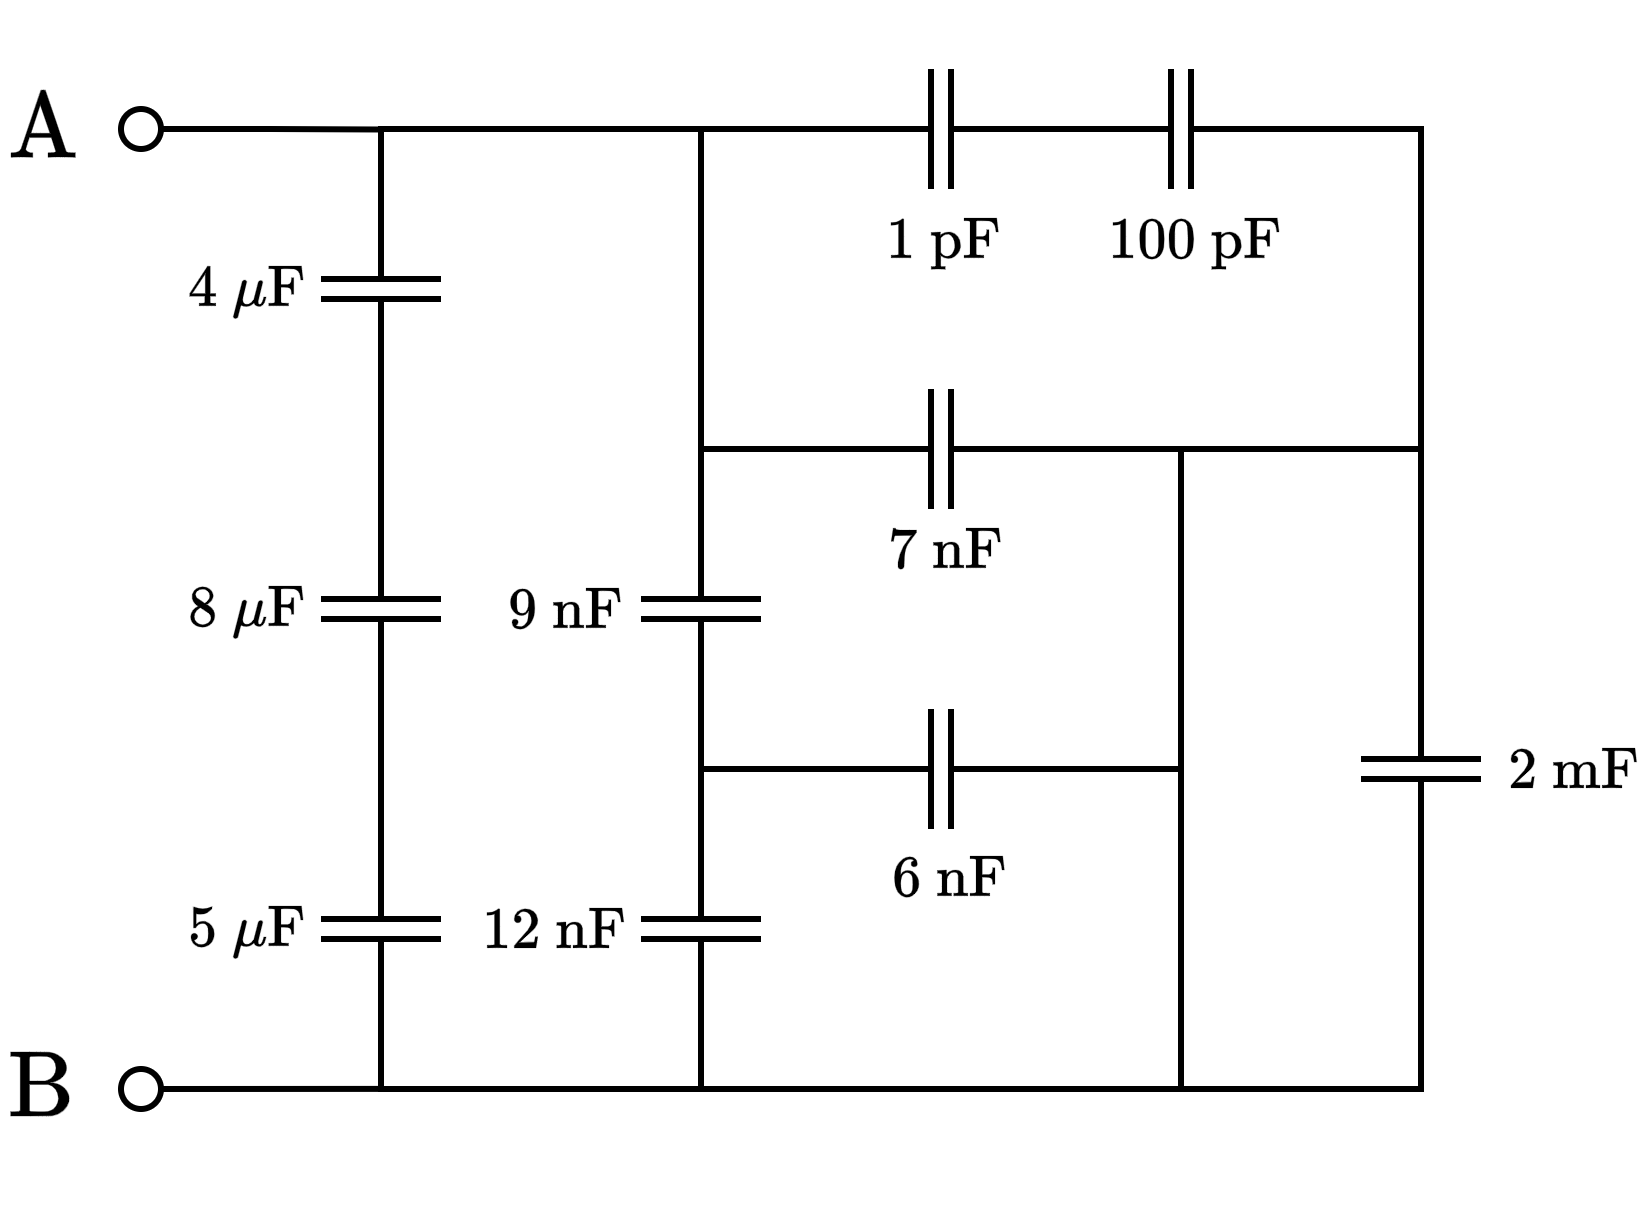
\includegraphics[width=0.8\textwidth]{questionbank/circuit_quantities/capacitor_network/v1/network_diagram.png}
\end{center}

% =========================================================
\begin{partquestion}{networksteadycurrent}
{Calculate the steady-state current through each capacitor if a \qty{12}{\volt} battery is placed between A and B.}

\begin{answer}
At steady state, each capacitor will act like an open circuit and there will be no current through any of the capacitors. Therefore, all capacitor currents are zero.
\end{answer}
\end{partquestion}

% =========================================================
\begin{partquestion}{networksteadyvoltage}
{Calculate the voltage across each capacitor if a \qty{12}{\volt} battery is placed between A and B. Label the capacitor network with the voltages you found. Assume the higher potential is connected to node A.}

\begin{answer}
The voltage is a little more complicated, but there are still some easy ones. Notice how the 7nF capacitor is connected directly to both A and B. This means it's in parallel with the battery so its voltage
\[V_{C7} = \qty{12}{\volt}\]
The next easy one is our 2mF capacitor out on the right. Notice that both of its terminals are connected to B. Since an ideal wire connects both sides of the capacitor, it's not possible for it to hold any voltage, it has been 'shorted out', so its voltage \[V_{C2} = \qty{0}{\volt}\]
Next let's attack the 1pF and 100pF capacitors up near the top. KVL lets us recognize that the sum of their voltages should add up to the battery voltage
\[V_{C1} + V_{C100} = \qty{12}{\volt}\]
Additionally, they also share current since they are in series. Since the current is the rate of change of charge, this also implies they store the same total charge $Q_{C1} = Q_{C100}$ (assuming no charge was stored before we started). Using the definition of charge on a capacitor we can write
\[C_1V_{C1}=C_{100}V_{C100}\]
Combining with the previous equation:
\begin{align*}
V_{C1} + \frac{C_{1}}{C_{100}}V_{C1} &= 12 \\
V_{C1} &= \frac{12C_{100}}{C_1 + C_{100}} \\
V_{C1} &= \frac{\qty{12}{\volt}\cdot\qty{100}{\pico\farad}}{\qty{1}{\pico\farad} + \qty{100}{\pico\farad}} = \frac{\qty{1200}{\volt\pico\farad}}{\qty{101}{\pico\farad}} \approx 11.9\text{ V} \\
V_{C100} &= 12 - V_{C1} \\
V_{C100} &\approx 12 - 11.9 = \qty{0.1}{\volt}
\end{align*}
Interesting, notice that most of the voltage is on the smaller capacitor. That's the reverse of what we see in a resistive voltage divider, where the larger resistor has most of the voltage across it. Also take note that the units of \unit{\pico\farad} canceled out. More generally, this shows that it's the ratio of the capacitance values that matters here, not the magnitude of the capacitance. Hence in future calculations we can neglect the units if they are all the same.

Let's take the string of three capacitors on the right, now that we know how to handle capacitors in series. As before we can write $Q_{C4} = Q_{C8} = Q_{C5} = Q_{string}$ and $V_{C4} + V_{C8} + V_{C5} = 12$. This time, let's set up the equation a little differently by recognizing that $V = Q/C$. This lets us write the following:
\begin{align*}
\frac{Q_{C4}}{C_4} + \frac{Q_{C8}}{C_8} + \frac{Q_{C5}}{C_5} &= 12 \\
Q_{string}(\frac{1}{C_4} + \frac{1}{C_8} + \frac{1}{C_5}) &= 12 \\
Q_{string} &= \frac{12}{(\frac{1}{C_4} + \frac{1}{C_8} + \frac{1}{C_5})} \\
Q_{string} &= \frac{12}{(\frac{1}{\qty{4}{\micro\farad}} + \frac{1}{\qty{8}{\micro\farad}} + \frac{1}{\qty{5}{\micro\farad}})} \\
Q_{string} &= \qty{12}{\volt} \cdot \frac{40}{23}\unit{\micro\farad} = \frac{480}{23}\unit{\micro\coulomb}
\end{align*}

Now that we have $Q_{string}$ we can solve for each capacitor voltage directly using $V = Q/C$.
\begin{align*}
    V_{C4} &= \frac{Q_{string}}{C_4} = \frac{\frac{480}{23}\unit{\micro\coulomb}}{\qty{4}{\micro\farad}} = \frac{120}{23} \approx \qty{5.22}{\volt} \\
    V_{C8} &= \frac{Q_{string}}{C_8} = \frac{\frac{480}{23}\unit{\micro\coulomb}}{\qty{8}{\micro\farad}} = \frac{60}{23} \approx \qty{2.61}{\volt} \\
    V_{C5} &= \frac{Q_{string}}{C_5} = \frac{\frac{480}{23}\unit{\micro\coulomb}}{\qty{5}{\micro\farad}} = \frac{96}{23} \approx \qty{4.17}{\volt}
\end{align*}
As a sanity check, we can show that $5.22 + 2.61 + 4.17 = 12$. Notice again how the largest voltage is across the smallest capacitor.

The last remaining voltages to be found are for the 9nF, 6nF and 12nF capacitors in the middle. This looks more complicated since this isn't a simple series string of capacitors. However, we can use parallel combinations to simplify the problem. Since the 12nF and 6nF capacitors are in parallel, they will share the same voltage! That means we can combine them into one capacitor without losing access to the variables we care about. Capacitors simply add in parallel $\qty{12}{\nano\farad} + \qty{6}{\nano\farad} = \qty{18}{\nano\farad}$, so we will place an effective 18nF cap in the place of the 6nF and 12nF. Now we have the same situation as before, with $C_9$ in series with $C_{18}$.

\begin{align*}
V_{C9} + \frac{C_{9}}{C_{18}}V_{C9} &= 12 \\
V_{C9} &= \frac{12C_{18}}{C_9 + C_{18}} \\
V_{C9} &= \frac{12 \cdot 18}{9 + 18} = \frac{216}{27} = \qty{8}{\volt} \\
V_{C18} &= 12 - V_{C9} \\
V_{C18} &= 12 - 8 = \qty{4}{\volt} \\
\end{align*}

Recalling that the voltage across our $C_{18}$ combo will be the same as it's original parts, we have
\[V_{C6} = V_{C12} = \qty{4}{\volt}\]

We can now summarize our results for our own tidiness and then relabel the original schematic as required. Since the higher potential is at node A, we label each capacitor with the positive end towards node A since that must have been where the charging current originated from.

\begin{table} [h]
    \centering
    \begin{tabular}{| c | c |}
        \hline
        Capacitor & Voltage \\ \hline
        $C_{1}$ & 11.9 \\
        $C_{2}$ & 0 \\
        $C_{4}$ & 5.22 \\
        $C_{5}$ & 4.17 \\
        $C_{6}$ & 4 \\
        $C_{8}$ & 2.61 \\
        $C_{7}$ & 12 \\
        $C_{9}$ & 8 \\
        $C_{12}$ & 4 \\
        $C_{100}$ & 0.1 \\
        \hline
    \end{tabular}
\end{table}

\begin{center}
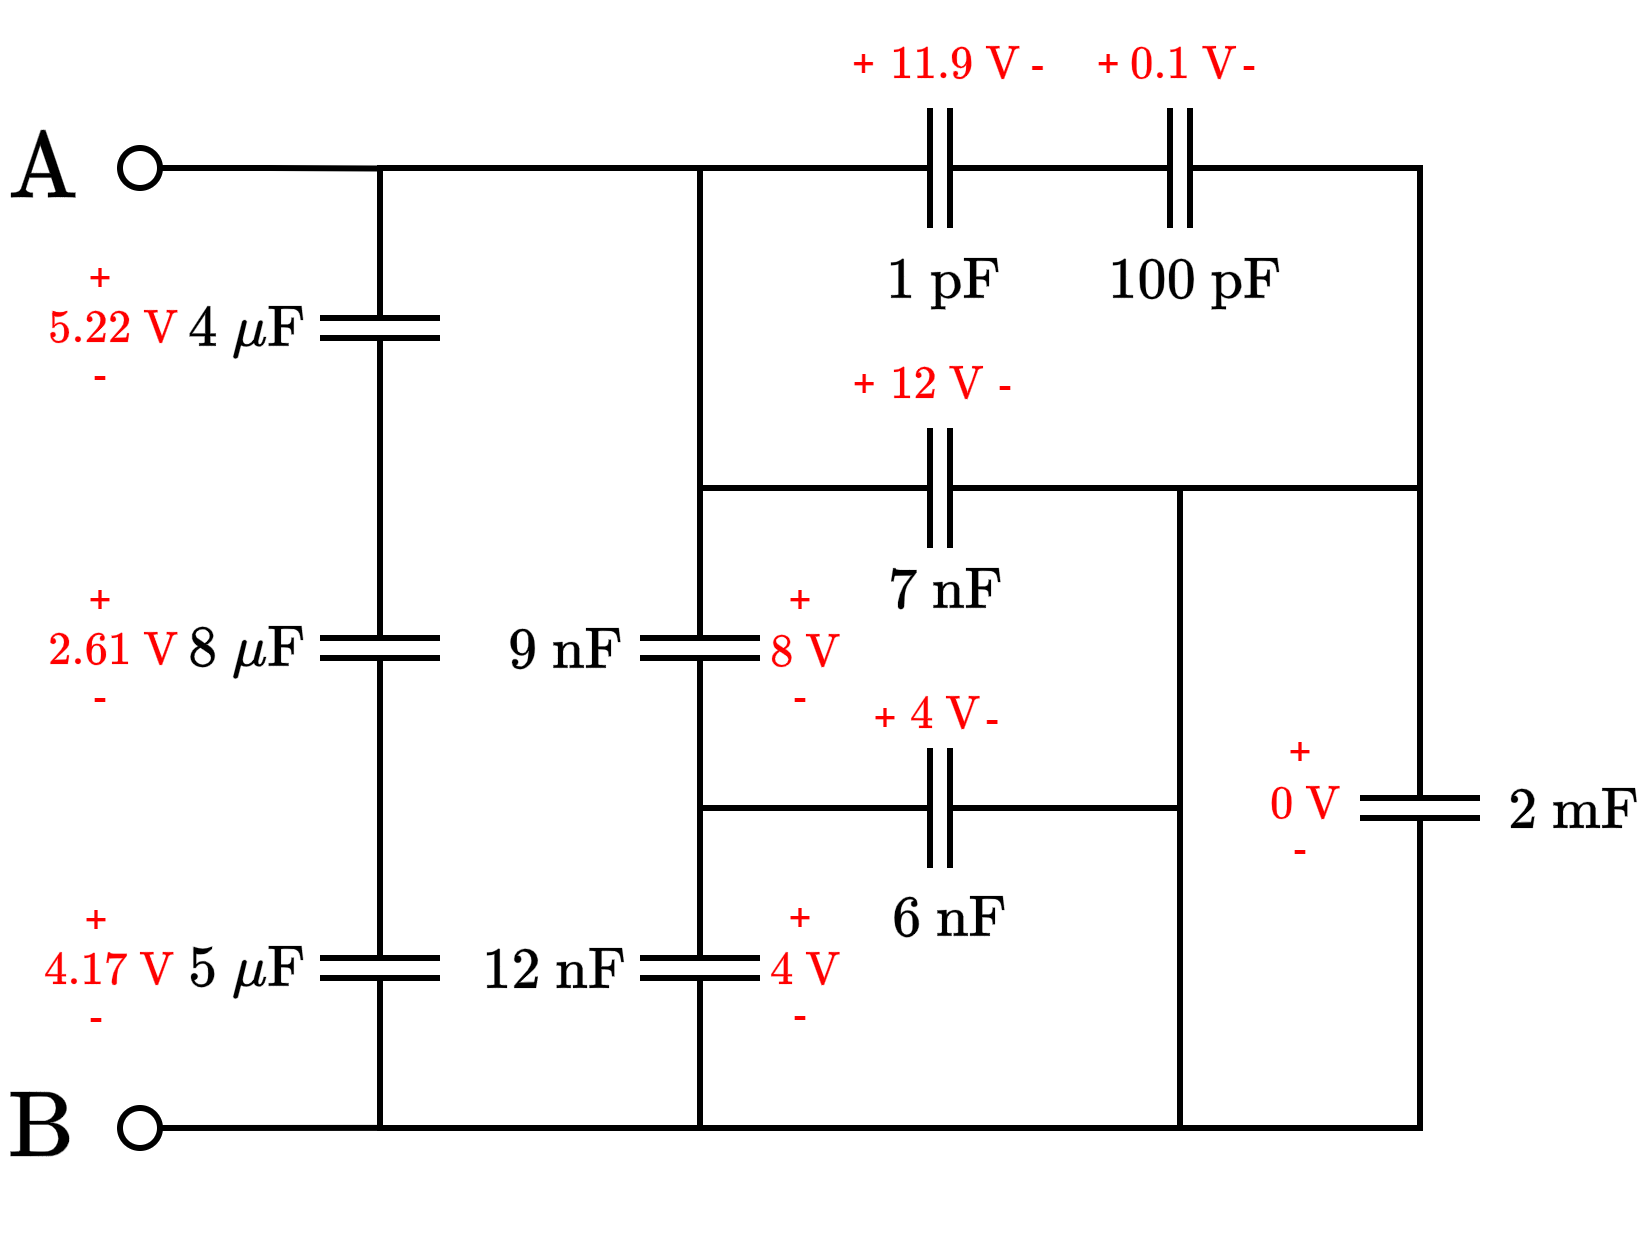
\includegraphics[width=0.8\textwidth]{questionbank/circuit_quantities/capacitor_network/v1/network_diagram_sol.png}
\end{center}

\end{answer}
\end{partquestion}

\begin{partquestion}{energy}
{Which capacitor stores the most energy in part (\cref{prob:capacitornetwork:networksteadyvoltage})?}

\begin{answer}
    The energy in a capacitor is $E_C = \frac{1}{2}CV^2$. Since energy scales with capacitance, let's check the largest capacitors first. The \qty{2}{\milli\farad} cap will not store any energy since it has \qty{0}{\volt} across it. Let's compare the energy stored in the \unit{\micro\farad} capacitors.

    \begin{table} [h]
    \centering
    \begin{tabular}{| c | c | c |}
        \hline
        Capacitor & Voltage (V) & Energy (\unit{\micro\joule)} \\ \hline
        \textcolor{red}{$C_{4}$} & \textcolor{red}{5.22} & \textcolor{red}{54.5}\\
        $C_{5}$ & 4.17 & 43.5\\
        $C_{8}$ & 2.61 & 27.2\\
        \hline
    \end{tabular}
\end{table}

Looks like $C_4$ stores the most energy. We don't need to consider any of the other capacitors since they are all at least $\times1000$ smaller. Even if they were charged to the maximum battery voltage, that would only scale up the energy by $12^2 = \times144$. This guarantees they are smaller.

    
\end{answer}
\end{partquestion}

\end{mainquestion}


% Problem 3 - Capacitor and Inductor Experiment (20 points)
\clearpage
\Point{c_and_l_experiment}{current0}{3}
\Point{c_and_l_experiment}{currentt}{4}
\Point{c_and_l_experiment}{cap}{6}
\Point{c_and_l_experiment}{ratio}{3}
\Point{c_and_l_experiment}{energy}{4}
\Point{c_and_l_experiment}{charge}{3}
\MarkExtraCredit{c_and_l_experiment}{charge}
\begin{mainquestion}{c_and_l_experiment}{Capacitor and Inductor Experiment}
Your lab partner was experimenting with the following circuit:

\begin{center}
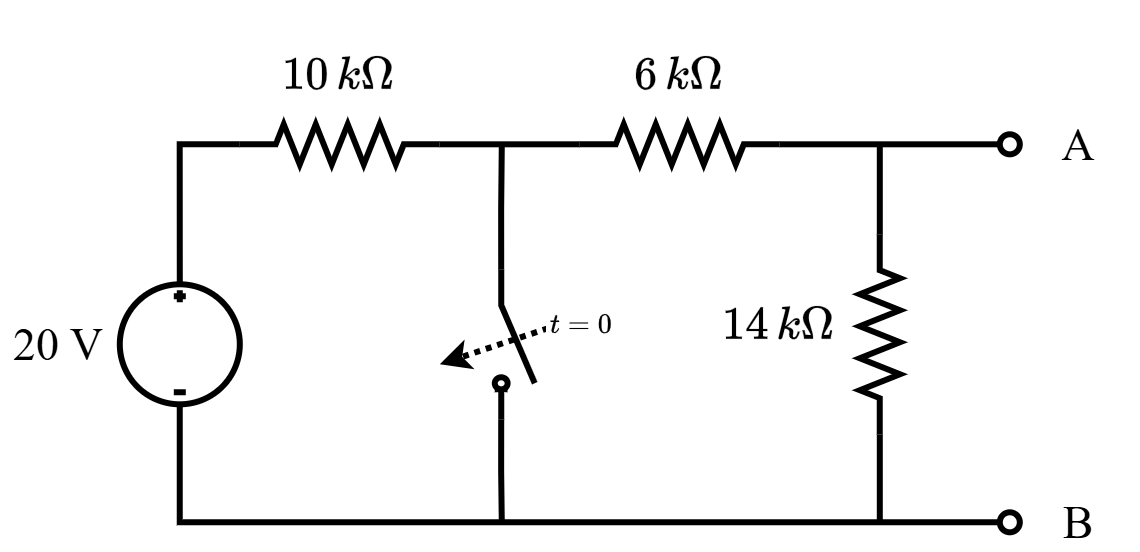
\includegraphics[width=0.8\textwidth]{questionbank/capacitors_and_inductors/c_and_l_experiment/v0/figure1.png}
\end{center}
They connected a \SI{300}{\milli\henry} inductor between terminals A and B, and left it hooked up for quite some time.

\begin{partquestion}{current0}{What is the current through the inductor $i_L(0^-)$?}
\begin{answer}
At DC, the inductor acts like a short. It follows that
\begin{align*}
 i_L(0^-)
 &= \frac{\SI{20}{\volt}}{\SI{10}{\kilo\ohm}+\SI{6}{\kilo\ohm}} \\
 &= \SI{1.25}{\milli\ampere}.
\end{align*}
\end{answer}
\end{partquestion}
\begin{partquestion}{currentt}{Your partner wants to find the inductor's current behavior. If the switch is closed at time $t=0$ seconds, what is the current through the inductor $i_L(t)$ for time $t>0$?}
\begin{answer}
After the switch is closed, the circuit looks as follows:
\begin{center}
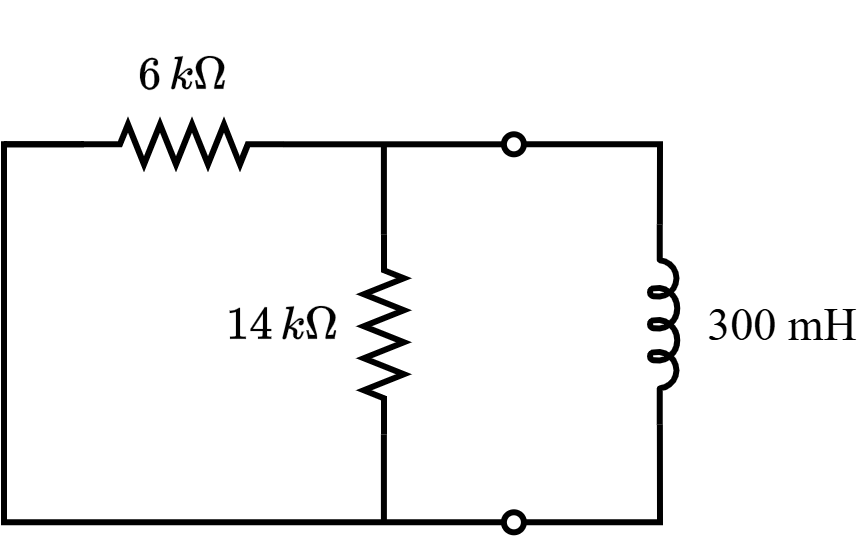
\includegraphics[width=0.8\textwidth]{questionbank/capacitors_and_inductors/c_and_l_experiment/v0/figure2.png}
\end{center}
The current through the inductor will decay exponentially based on the time constant according to
\begin{equation*}
 i_L(t)=i_L(0^-)e^{-t/\tau_L},
\end{equation*}
where
\begin{align*}
 \tau_L
 &= \frac{L}{R_{\mathrm{eq}}} \\
 &= \frac{\SI{0.300}{\henry}}
 {\SI{6}{\kilo\ohm}\parallel\SI{14}{\kilo\ohm}} \\
 &= \frac{(\SI{0.300}{\henry})(\SI{20}{\kilo\ohm})}
 {\SI{84}{\kilo\ohm\squared}} \\
 &= \SI{7.14e-5}{\second}.
\end{align*}
This gives
\begin{equation*}
 \boxed{i_L(t)=(\SI{1.25}{\milli\ampere})e^{-t/(\SI{7.14e-5}{\second})}},
 \qquad t>0.
\end{equation*}


\end{answer}
\end{partquestion}
\begin{partquestion}{cap}{You find an unmarked capacitor on the bench. You remove the inductor, open the switch again, and place the mysterious capacitor between terminals A and B and leave it hooked up for quite some time. You measure the voltage across the capacitor $v_C(t)$ after you close the switch at the start of your analysis, which we can again call $t=0$. Incredibly, it is a scaled copy of your partner's graph of $i_L(t)$. What is the value $C$ of the capacitor?}
\begin{answer}
At DC, the capacitor acts like an open. It follows that
\begin{align*}
 v_C(0^-)
 &= \frac{\SI{14}{\kilo\ohm}}
 {\SI{10}{\kilo\ohm}+\SI{6}{\kilo\ohm}+\SI{14}{\kilo\ohm}}
 (\SI{20}{\volt}) \\
 &= \SI{9.33}{\volt}.
\end{align*}

After the switch is closed, the circuit looks as follows:
\begin{center}
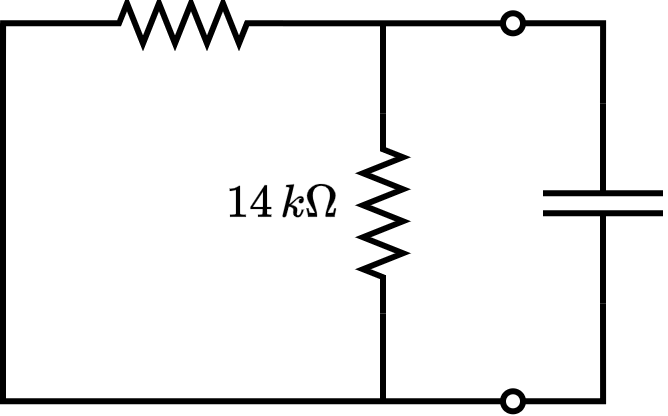
\includegraphics[width=0.8\textwidth]{questionbank/capacitors_and_inductors/c_and_l_experiment/v0/figure3.png}
\end{center}
The voltage across the capacitor will decay exponentially based on the time constant according to
\begin{equation*}
 v_C(t)=v_C(0^-)e^{-t/\tau_C},
\end{equation*}
where
\begin{equation*}
 \tau_C=R_{\mathrm{eq}}C
 =\left(\SI{6}{\kilo\ohm}\parallel\SI{14}{\kilo\ohm}\right)C.
\end{equation*}
For this to have the exact same shape, the exponential terms must be identical, which means that the time constants are also equal:
\begin{equation*}
 \tau_L=\tau_C.
\end{equation*}
This implies
\begin{align*}
 \left(\SI{6}{\kilo\ohm}\parallel\SI{14}{\kilo\ohm}\right)C
 &= \SI{7.14e-5}{\second}, \\
 C
 &= \frac{\SI{7.14e-5}{\second}}{\SI{4200}{\ohm}} \\
 &\approx \boxed{\SI{17}{\nano\farad}}.
\end{align*}

Did you see that coming?
\end{answer}
\end{partquestion}
\begin{partquestion}{ratio}{What is the ratio $v_C(t)/i_L(t)$ (with units)? What is the significance of this ratio? }
\begin{answer}
Because the two waveforms have identical exponential factors,
\begin{align*}
 \frac{v_C(t)}{i_L(t)}
 &= \frac{v_C(0^-)}{i_L(0^-)} \\
 &= \frac{\SI{9.33}{\volt}}{\SI{1.25}{\milli\ampere}} \\
 &= \boxed{\SI{7.47}{\kilo\ohm}}.
\end{align*}
This ratio is just the Th\'evenin resistance as seen by the load before the switch is thrown.
\end{answer}
\end{partquestion}
\begin{partquestion}{energy}{Find the approximate energy lost by your lab partner's inductor \SI{500}{\micro\second} after the switch was closed in part (\cref{prob:c_and_l_experiment:currentt}). Find the approximate energy lost by your capacitor \SI{500}{\micro\second} after the switch was closed in part (\cref{prob:c_and_l_experiment:cap}). In both cases, state where this energy went.}
\begin{answer}
\SI{500}{\micro\second} is more than five time constants, so we can assume that the inductor current and capacitor voltage have both reached zero by that time, and that each has lost all the energy it originally had when the switch was thrown.

For the inductor,
\begin{align*}
 E_L
 &= \frac{1}{2}L\left[i_L(0^-)\right]^2 \\
 &= \frac{1}{2}(\SI{0.300}{\henry})
    (\SI{0.00125}{\ampere})^2 \\
 &= \boxed{\SI{234}{\nano\joule}}.
\end{align*}

For the capacitor,
\begin{align*}
 E_C
 &= \frac{1}{2}C\left[v_C(0^-)\right]^2 \\
 &= \frac{1}{2}(\SI{17e-9}{\farad})(\SI{9.33}{\volt})^2 \\
 &\approx \boxed{\SI{740}{\nano\joule}}.
\end{align*}

In both cases, all the energy was absorbed in the \SI{6}{\kilo\ohm} and \SI{14}{\kilo\ohm} resistors and converted to heat.
\end{answer}
\end{partquestion}
\begin{partquestion}{charge}{Find the total charge that flows through the inductor in the first \SI{170}{\micro\second} after the switch closes in part (\cref{prob:c_and_l_experiment:currentt}).}
\begin{answer}
\begin{align*}
 Q
 &= \int_0^{\SI{170}{\micro\second}} i_L(t)\,dt \\
 &= \int_0^{\SI{170}{\micro\second}}
 (\SI{0.00125}{\ampere})e^{-t/(\SI{7.14e-5}{\second})}\,dt \\
 &= -\left(\SI{7.14e-5}{\second}\right)
    (\SI{0.00125}{\ampere})
    e^{-t/(\SI{7.14e-5}{\second})}
    \bigg|_0^{\SI{170}{\micro\second}} \\
 &\approx \SI{8.1e-8}{\coulomb} \\
 &= \boxed{\SI{81}{\nano\coulomb}}.
\end{align*}
\end{answer}
\end{partquestion}
\end{mainquestion}

% Problem 4 - Ideal Transformer Power Transfer and Transmission Lines (22 points)
\clearpage
\Point{transformerpowertransfer}{resistancetransformation}{3}
\Point{transformerpowertransfer}{directtransmission}{5}
\Point{transformerpowertransfer}{withstepuptransformers}{8}
\Point{transformerpowertransfer}{comparisonimplications}{2}
\Point{transformerpowertransfer}{dcsource}{4}
\begin{mainquestion}{transformerpowertransfer}{Ideal Transformer Power}

Consider the ideal transformer circuit shown below:

\begin{center}
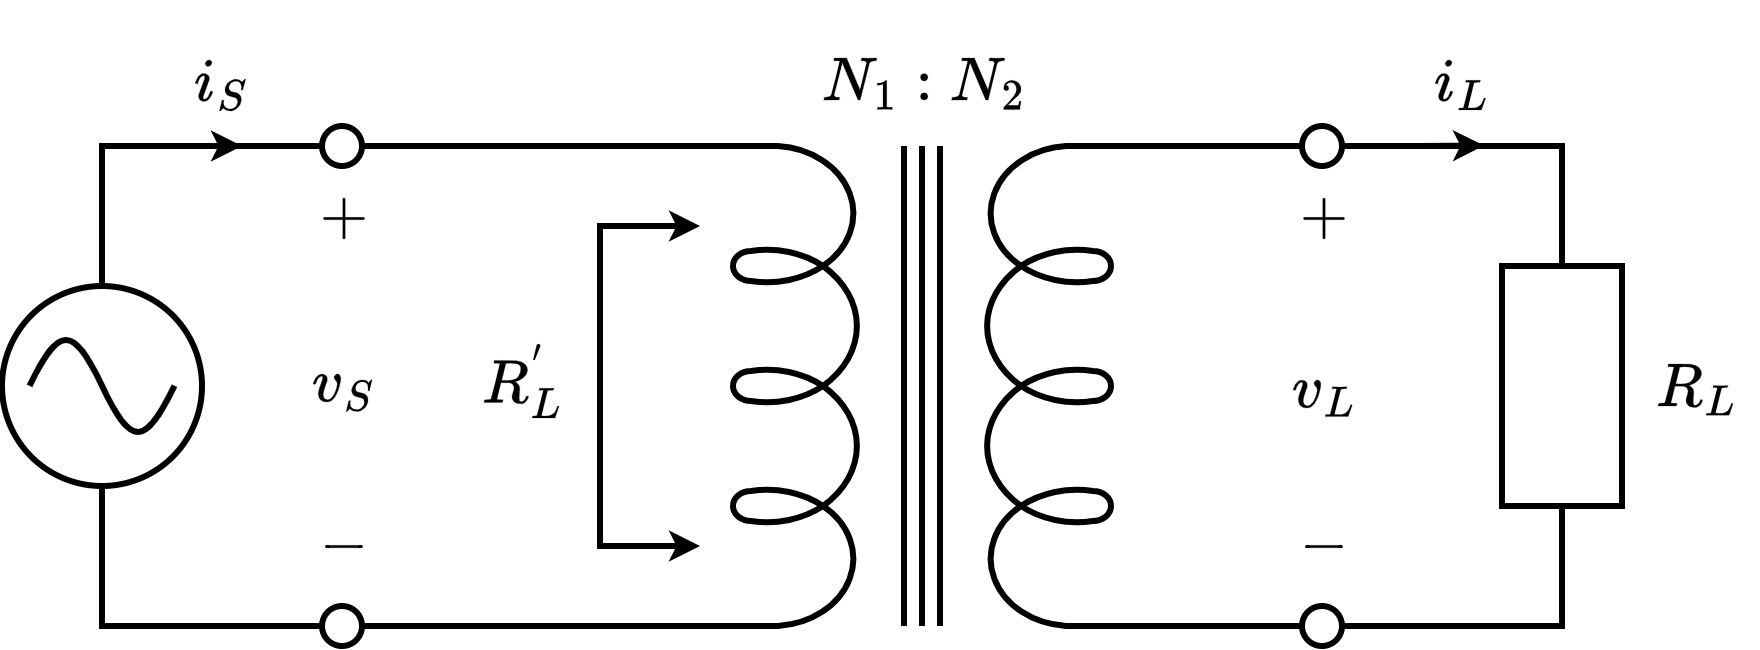
\includegraphics[width=0.8\textwidth]{questionbank/networks/transformer_power_transfer/v1/XFOR_symbolic.png}
\end{center}

% =========================================================
\begin{partquestion}{resistancetransformation}
{Derive the resistance $R_L' = v_S / i_S$ seen by the source, assuming an ideal transformer. This is a simple \emph{resistance transformation} across the transformer.}

\begin{answer}
From the definition of an ideal transformer:
\[
\frac{v_L}{v_S} = \frac{N_2}{N_1} \quad \text{and} \quad \frac{i_L}{i_S} = \frac{N_1}{N_2}
\]

It is straightforward to show that:

\[
R_L' \equiv \frac{v_S}{i_S} = \frac{v_L(N_1/N_2)}{i_L(N_2/N_1)} = \frac{v_L}{i_L}\left(\frac{N_1}{N_2}\right)^2 = R_L\left(\frac{N_1}{N_2}\right)^2
\]

The resistance as seen from the primary side is scaled by the square of the turns ratio.
\end{answer}
\end{partquestion}

% =========================================================
\begin{partquestion}{directtransmission}
{Consider a 340 V peak-to-peak sinusoidal source connected to a resistive load of 17 $\Omega$ via a transmission line without transformers, having a total line resistance of 17 $\Omega$. Determine the power delivered by the source, the power dissipated in the line, the power delivered to the load, and the efficiency $\eta = P_{\text{load}} / P_{\text{source}} \times 100\%$.}

\begin{center}
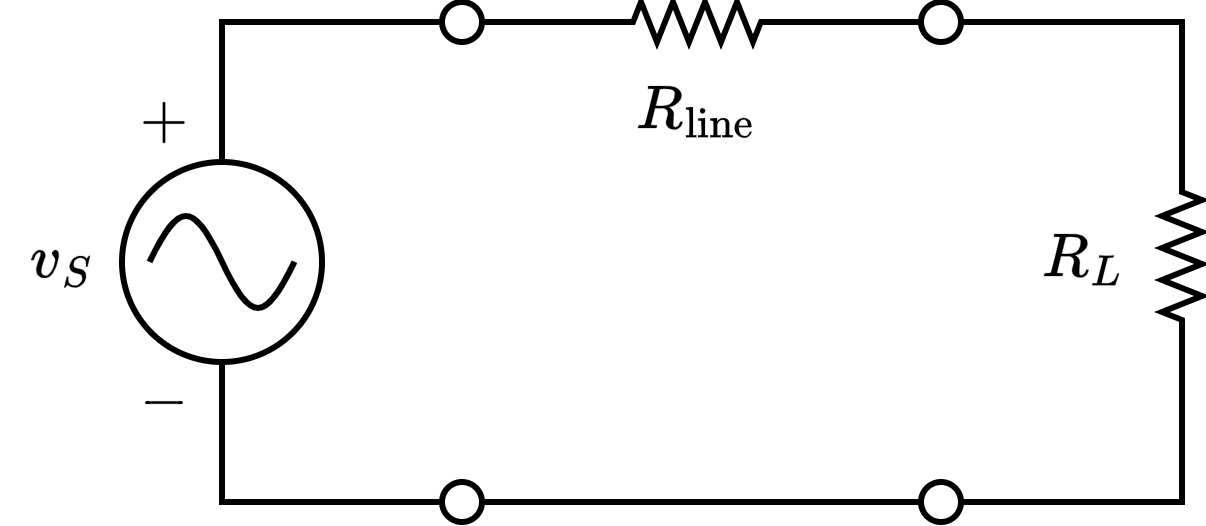
\includegraphics[width=0.6\textwidth]{questionbank/networks/transformer_power_transfer/v1/XFOR_matched.png}
\end{center}

\begin{answer}
The power delivered by the source is $P = v_{\text{source,rms}}^2 / (R_{\text{line}} + R_L)$. The voltage is given as peak-to-peak, so the amplitude is 170~V and the RMS value is $170/\sqrt{2}$~V $\approx 120$~V.

\[
P_{\text{delivered}} = \frac{v_{s,\text{rms}}^2}{R_{\text{line}} + R_L} = \frac{120^2}{17 + 17} = \frac{14400}{34} \approx 424\text{ W}
\]

The power dissipated in the line is:

\[
P_{\text{line}} = \frac{v_{\text{line,rms}}^2}{R_{\text{line}}} = \left(\frac{R_{\text{line}}}{R_{\text{line}} + R_L} v_{\text{source, rms}}\right)^2 \frac{1}{R_{\text{line}}} = \left(\frac{17}{34} \cdot 120\right)^2 \frac{1}{17} = \frac{3600}{17} = 212\text{ W}
\]

The remaining power is dissipated in the load:

\[
P_{\text{load}} = 424\text{ W} - 212\text{ W} = 212\text{ W}
\]

The efficiency is:

\[
\eta = \frac{212\text{ W}}{424\text{ W}} \times 100\% = 50\%
\]

This circuit delivers maximum power transfer to the load because line resistance is equal to that of the source resistance.
\end{answer}
\end{partquestion}

% =========================================================
\begin{partquestion}{withstepuptransformers}
{Now introduce a pair of transformers: a step-up transformer (1:10) before the transmission line and a step-down transformer (10:1) after the transmission line, as shown below. Using the result from part (\cref{prob:transformerpowertransfer:resistancetransformation}), transform the resistance to the source side of the transformer and again determine the power delivered by the source, the power dissipated in the line, the power delivered to the load, and the efficiency. Is this circuit delivering maximum power transfer to the load (which in this case occurs when the load resistance when transformed across the step-down transformer is equal to the line resistance)?}

\begin{center}
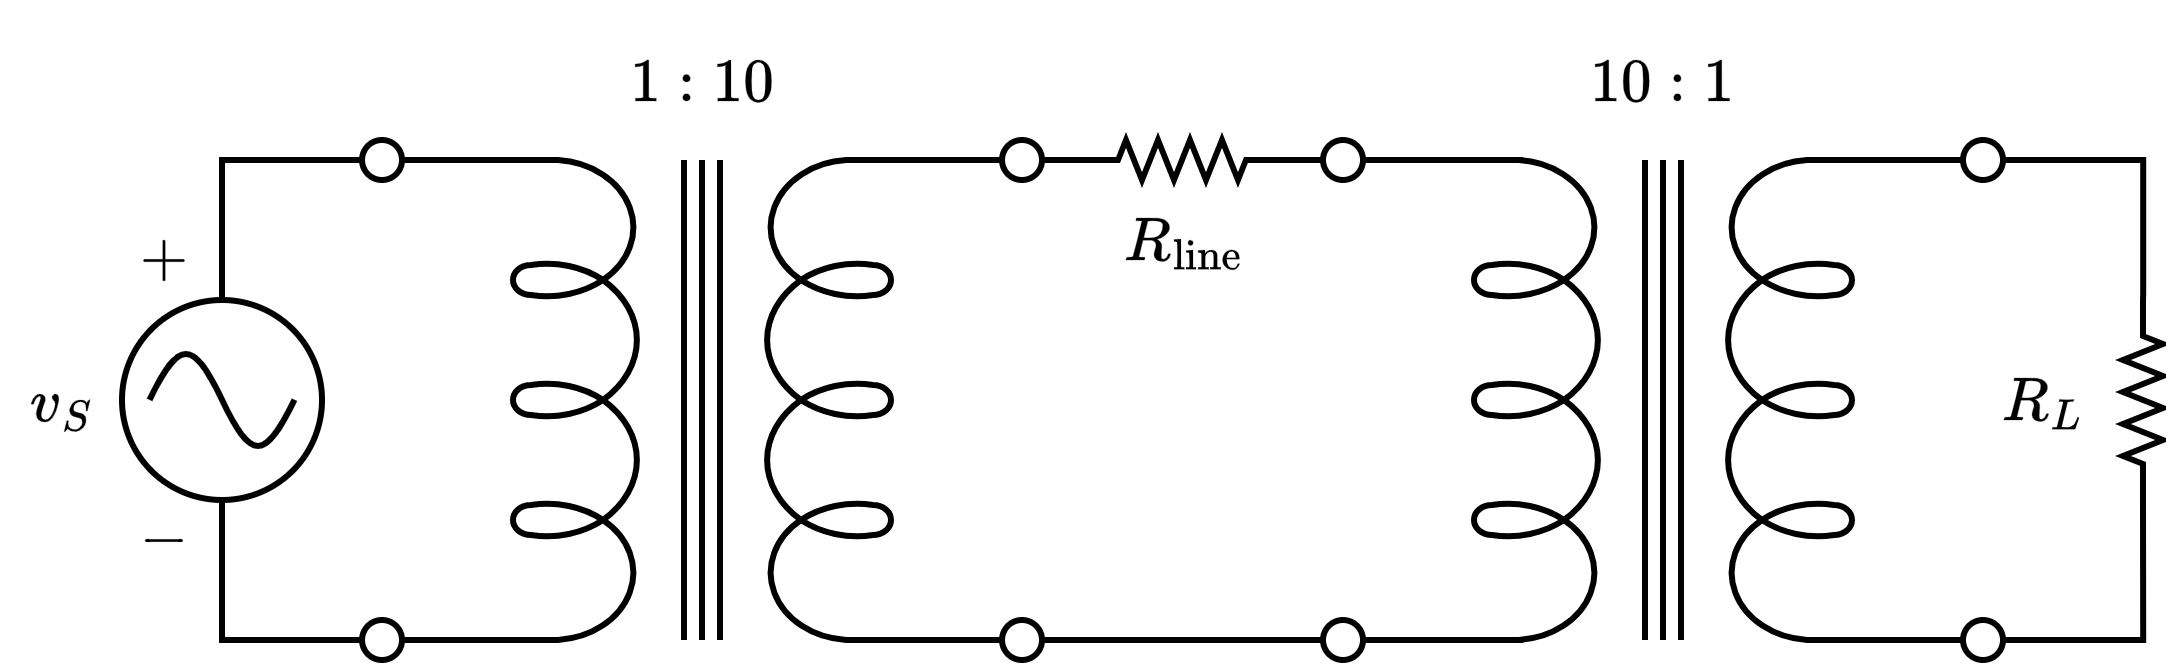
\includegraphics[width=0.9\textwidth]{questionbank/networks/transformer_power_transfer/v1/XFOR_step.png}
\end{center}

\begin{answer}
The load needs to be transformed across the step-down transformer, and then both resistors need to be transformed across the step-up transformer.

First resistance transformation (load across step-down transformer):

\[
R_L'' = R_L \left(\frac{10}{1}\right)^2 = 100 R_L = 1700\text{ }\Omega
\]

Second resistance transformation (both resistors across step-up transformer):

\[
R_L' = \left(R_{\text{line}} + R_L''\right) \left(\frac{1}{10}\right)^2 = \frac{R_{\text{line}}}{100} + R_L = \frac{17}{100} + 17 = 17.17\text{ }\Omega
\]

The power delivered is:

\[
P_{\text{delivered}} = \frac{120^2}{0.17 + 17} \approx 839\text{ W}
\]

The power dissipated in the line (which now sees voltage stepped up by factor of 10):

\[
P_{\text{line}} = \frac{[v_{\text{source,rms}} \cdot \frac{R_{\text{line}}/100}{ R_{\text{line}}/100 + R_L}]^2}{R_{\text{line}}/100} = \frac{120^2(17/100)}{(17/100 + 17)^2} \approx 8.30\text{ W}
\]

The remaining power is dissipated in the load:

\[
P_{\text{load}} = \qty{839}{\watt} - \qty{8.30}{\watt} \approx \qty{830.4}{\watt}
\]

The efficiency is:

\[
\eta = \frac{\qty{830.4}{\watt}}{\qty{839}{\watt}} \times 100\% = 99\%
\]

This circuit is \textbf{not} delivering maximum power transfer to the load because the line resistance is not equal to that of the (transformed) load
resistance.
\end{answer}
\end{partquestion}

% =========================================================
\begin{partquestion}{comparisonimplications}
{Comparing answers to parts (\cref{prob:transformerpowertransfer:directtransmission}) and (\cref{prob:transformerpowertransfer:withstepuptransformers}), what do your results indicate?}

\begin{answer}
The use of a transformer pair to step up and step down the voltage provides a much more efficient mechanism to transport power over transmission lines. The efficiency improved from 50\% to 99\% by using transformers to step up voltage before transmission and step down after. Note that greater efficiency does not imply that the maximum power is being transferred!
\end{answer}
\end{partquestion}

% =========================================================
\begin{partquestion}{dcsource}
{Will your results be the same in parts (\cref{prob:transformerpowertransfer:directtransmission}) and (\cref{prob:transformerpowertransfer:withstepuptransformers}) if the source is replaced by a 340 V DC battery? What about the efficiency? Explain your answers.}

\begin{answer}
For part (\cref{prob:transformerpowertransfer:directtransmission}), not quite, since the original AC voltage source was 340 V peak-to-peak. An equivalent DC battery from a power perspective would be one operating at $120$~V.

For part (\cref{prob:transformerpowertransfer:withstepuptransformers}), not at all, because transformers block all DC voltages from propagating down the transmission line. There will be no power dissipated in the load (or the line!).
\end{answer}
\end{partquestion}

\end{mainquestion}


